\chapter{Data Distribution Service}
\section{Overview}


\section{Middleware}
\subsection{What and why?}


\begin{center}
	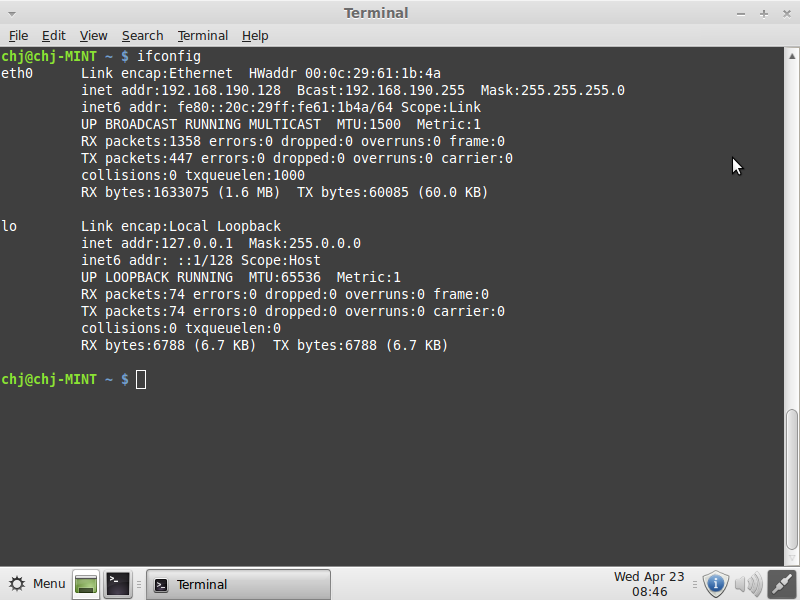
\includegraphics[width=\textwidth]{ifconfig.png}
	\captionof{figure}{Eksempel på billede}
\end{center}

\subsection{Decoupling}



\subsection{Publish/Subscribe pattern}


\subsection{Real-time systems}

\section{Quality Of Service}
For setting up the connections between entities, Publishers, Middleware and Subscribers must agree on certain terms. Quality of Service (QoS) lets the middleware know how to treat connections between publishers and subscribers as well as how to treat messages.

The QoS lets us setup \textit{terms} of the communication. This can be used, for instance, to set up the \textit{lifetime} of a message. This way, we could make sure a message will stop being interesting to subscribers after a while. 

Another example is setting the \textit{deadline} parameter on a subscribers QoS. This tells publishers, that the subscriber expects data within the specified timeframe. This way, if the middleware detects a QoS of the publisher, which will transfer data at a slower rate than what the subscriber requests, the middleware will \textbf{not} connect these two.

The QoS can be set programmatically through properties and structs in the respective classes or through XML configuration files. 

\section{Connext RTI}

\subsection{Configuration on linux}